\section{Technical Overview}
\label{sec:technical_overview}
In this section, we give a high-level overview of our techniques.
First, Algorithm~\ref{alg:greedy} defines the greedy algorithm that we use in this paper.
Throughout this paper, we refer to Algorithm~\ref{alg:greedy} as $\greedy$.
Note that $\greedy$ exits as soon as the budget constraint is violated.

\begin{algorithm}
\caption{Greedy Algorithm ($\greedy$)}
\label{alg:greedy}
\begin{algorithmic}[1]
\State \textbf{Input}: price vector $\vec p$, values $\vec v$, budget $B$, feasible sets $\I \in 2^{[n]}$.
\State \textbf{Output}: set $G$ of modules.
\State Initialize $G \gets \emptyset$.
\State Re-arrange modules such that $\frac{\vecv(1)}{\vecp(1)} \geq \frac{\vecv(2)}{\vecp(2)} \geq \dots \geq \frac{\vecv(n)}{\vecp(n)}$ with ties broken arbitrarily.
\For{$i=1,2 \dots ,n$}
\If{$i \in \spn(G)$}
\State Let $C$ be the unique circuit in $G \cup \{i\}$.
\State Let $j \in \argmin\{ \vecv(j') \,:\, j' \in C\}$.
\State Set $G' \gets G \cup \{i\} \setminus \{j\}$.
\Else
\State Set $G' \gets G \cup \{i\}$.
\EndIf
\If{$\vecp(G') > B$}
\State \textbf{break}
\EndIf
\State $G \gets G'$.
\EndFor
\State \textbf{return} $G$
\end{algorithmic}
\end{algorithm}


\subsection{Existence of Equilibria}

In this paper, we will give constructive proofs that $\eps$-equilibria exist in the pricing game when the allocation rule is given by Algorithm~\ref{alg:greedy} (see the formal results and proofs in Section~\ref{subsec:eq_exists}, Section~\ref{sec:matroid_price_eqm_existance}, and Section~\ref{sec:weighted_matroid_equilibrium}).
In this section, we give a high-level intuition of how to make such constructions.
For simplicity, let us assume that the modules are sorted in increasing order of ``cost-per-value'' and that these values are distinct, i.e.~$\frac{\vecc(1)}{\vecv(1)} < \ldots < \frac{\vecc(n)}{\vecv(n)}$.
Note that this is equivalent to decreasing bang-per-buck order.

First, assume there is no matroid constraint.
At a high-level, the algorithm starts by assuming every module bids their cost.
However, this means that the module with the highest cost-per-value (the inverse of the bang-per-buck) can raise its bid since it is the first module inspected by $\greedy$.
So it increases its cost-per-value up until the next module inspected by $\greedy$.
Then the two modules, as a coalition, increase their price to the third module inspected by $\greedy$.
This process continues until a step $k$ where increasing modules $1, \ldots, k$ to the cost-per-value of module $k+1$ would cause the first $k+1$ modules to exceed the budget constraint.
When this happens, we instead raise the cost-per-value of the first $k$ modules as high as possible so that the first $k$ modules fit within the budget constraint.
We note that the set of module which increases their price remains selected by the greedy algorithm. In addition, increasing the price of these module can only decrease the utility of the rest of the module. Therefore, 
intuitively, this should be an equilibrium since no accepted module can increase their price while remaining accepted by $\greedy$ and no rejected module is willing to lower their price since it is already bidding its cost.

The argument becomes more complex when a matroid constraint is introduced.  Imagine we try to iteratively increase the prices of the modules, similar to how we did in the additive case. With a matroid constraint, a module (or set of modules) might have its price increased and still be selected by the greedy algorithm.  This price update, however, could cause the algorithm to drop a module with the lowest bang-per-buck (due to the matroid constraint) and swap it for a module with a higher bang-per-buck that wasn't previously selected at the original price.

This means that modules rejected earlier during the price update process can suddenly become ``important'' and might be willing to increase their prices in future updates.  This ``non-monotonic'' behavior makes things tricky. To handle this, we have carefully designed an algorithm (Algorithm~\ref{alg:equilibrium_dynamics_weighted}) that keeps track of these modules that are suddenly selected. In our equilibrium construction, we make sure that if such modules exhibit profitable price deviations, we update their prices accordingly. 

Figure~\ref{fig:matroidAlg} illustrates a sample run of this process for unweighted matroid using the graphic matroid shown in the top left.
In other words, the goal is to pick a subset of the edges with the constraint that no cycle is formed. We note that the unweighted case does satisfies certain nice monotonicity properties (Claim~\ref{claim:winners_stays_winners}) which is not present in the weighted case which requires more careful technical treatment for the quality of equlibria. 

In Figure~\ref{fig:matroidAlg}, each point corresponds to a module.
The value above the module is the name of the module while the coordinates below the module correspond to the value and price, respectively, of the module.
Each plot corresponds to a separate step $t$ for the construction of the equilibrium.
In addition, each plot only shows what $\greedy$ would do up until iteration $t$.
Question marks correspond to modules that have not been reached at the current step of the construction.
The \textcolor{blue}{blue dots} indicate modules \textcolor{blue}{accepted} by $\greedy$ by its $t$ iteration and \textcolor{red}{red crosses} indicate modules \textcolor{red}{rejected} by $\greedy$ by its $t$th iteration.

In the first three steps of the construction, we slowly raise the cost-per-value.
In each of these steps $t$, the first $t$ iterations of $\greedy$ ensures that all modules are accepted.
Let us now consider step $4$ of the construction and assume that $\greedy$ tie-breaks in lexicographic order.
In this case, $\greedy$ would start by accepting modules $1$, $2$, and $3$.
When it reaches module $4$, it would realize that $4$ forms a cycle with $1$ and $2$.
Module $1$ has the lowest value in the cycle so it is replaced by module $4$.
At this point, the price of module $1$ is moot but to better illustrate the operation of $\greedy$, we assume that it freezes at price.

Finally, let us look at step $5$.
The lowest cost-per-value module is module $1$.
So $\greedy$ begins by taking module $1$.
It then takes modules $2$ and $3$ and finally replaces $1$ with $4$.
Once it takes module $4$, the budget is exhausted and so $\greedy$ terminates.

Observe that the result in step $5$ is indeed an equilibrium.
Modules $2$, $3$, and $4$ cannot increase their prices since if they do, they would be fourth in the order and be rejected.
Module $1$ will always be replaced by $4$ whenever it becomes before $4$ and module $5$'s cost is too high for it be relevant.

\begin{figure}[h]
\centering
\begin{subfigure}{0.3\textwidth}
  \centering
  \scalebox{0.9}{
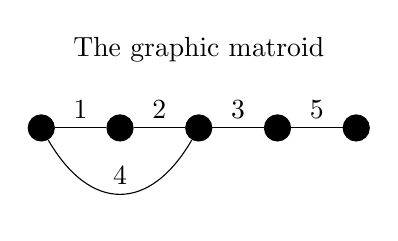
\begin{tikzpicture}[
    node distance=1cm
]
  \node[circle,draw,fill] (a) {};
  \node[circle,draw,fill,right of=a] (b) {};
  \node[circle,draw,fill,right of=b] (c) {};
  \node[circle,draw,fill,right of=c] (d) {};
  \node[circle,draw,fill,right of=d] (e) {};

  \draw (a) -- node[above] {1} (b);
  \draw (b) -- node[above] {2} (c);
  \draw (c) -- node[above] {3} (d);
  \draw (d) -- node[above] {5} (e);
  \draw (a) edge[bend right=60,looseness=1.5] node[above] {4} (c);
  
  \node[above of=c] {\normalsize The graphic matroid};
\end{tikzpicture}
}
\end{subfigure}%
\hfill
\begin{subfigure}{0.3\textwidth}
  \centering
  \plotWeightedMatroidIterationOne{\tikzscale}
\end{subfigure}%
\hfill
\begin{subfigure}{0.3\textwidth}
  \centering
  \plotWeightedMatroidIterationTwo{\tikzscale}
\end{subfigure}%

\medskip

\begin{subfigure}{0.3\textwidth}
  \centering
  \plotWeightedMatroidIterationThree{\tikzscale}
\end{subfigure}%
\hfill
\begin{subfigure}{0.3\textwidth}
  \centering
  \plotWeightedMatroidIterationFour{\tikzscale}
\end{subfigure}%
\hfill
\begin{subfigure}{0.3\textwidth}
  \centering
  \plotWeightedMatroidIterationFive{\tikzscale}
\end{subfigure}%
\caption{Sample run for equilibrium construction. See main text for description.}
\label{fig:matroidAlg}
\end{figure}


\subsection{Quality of Equilibria}
\paragraph{Characterizing worst-case equilibria.}
Our first step to prove approximation results of equilibria is to first characterize the set of ``worst-case'' equilibria.
We first prove a technical result that shows that in the worst-case equilibria, roughly speaking, all rejected modules bid their cost.
This statement is exactly true in the setting without a matroid constraint and in the setting with a matroid constraint but with uniform values.
For the setting with general values, this statement is only partly true and we can only make this characterization up to a single module; we will leave the technical details of this to Section~\ref{sec:weighted_matroid}.

Our overall approach is to demonstrate that, starting from any equilibrium price, we can reach another equilibrium through a sequence of price deviations.  This sequence will ensure that all "crucial" non-selected module sets have their prices equal to their costs, while simultaneously decreasing the total value for the platform. We then analyze the value of such equilibria using properties of the greedy algorithm, allowing us to directly compare it to the optimal value, OPT.

The main technical challenge lies in the following: once we update the price of a non-selected module to its cost, it can create several new potential profitable deviations for other modules. These deviations must be addressed to reach a new equilibrium without changing the price of the non-selected module we just adjusted.  Our core technical analysis focuses on tracking all these potential new deviations and arguing that our specific sequence of deviations ultimately leads to an equilibrium where the "crucial" non-selected modules have their prices set equal to their costs.


To give more high-level intuition of our approach, we start with an equilibrium price vector $\vecp$ and some module $i$ such that $\vecp(i) > \vecc(i)$.
We then decrease the price of module $i$ to $\vecc(i)$.
Note that module $i$ must remain rejected because otherwise it could have deviated in $\vecc(i)$.\footnote{Here, we ignore the edge case where module $i$ can be accepted with non-negative utility if and only if it bids $\vecc(i)$.}
Now consider the new price vector given by $(\vecc(i), \vecp_{-i})$.
Let $S$ denote the set of modules selected by $\greedy$ when $\greedy$ considers module $i$.
If $i$ is budget-feasible when $\greedy$ inspects it but is then rejected anyway then it turns out this is already an equilibrium.
The reason is as follows.
Observe that $i$'s deviation could result in one of two possibilities.
First, it could be that when $\greedy$ reaches module $i$, including $i$ would have already formed a circuit and module $i$ would be the least valuable module in that circuit.
The other is that $\greedy$ temporarily adds module $i$. In this case, it must be that module $i$ is later removed since it forms a circuit.
In both of these cases, the intuition is that the price of $i$ is somewhat moot (provided that it bids above its cost).
In which case, it did not really matter than $i$ had placed a bid above its cost in the first place.

The difficult case is when module $i$ could have been added to $S$ by $\greedy$ but was not added because doing so would violate the budget constraint.
This may cause modules after $i$ to now be rejected which were previously accepted.
To resolve this, we need a two-step process.
First, we modify the prices of all newly rejected modules so that their price is the greater of their own cost or the price given by module $i$'s current bang-per-buck.
Note that not all of these modules may be able to accept the new price.
This can allow some modules which come before $i$ and that were previously rejected to now be accepted.
These modules now have an incentive to deviate.
So the second step is to raise their prices up to the bang-per-buck of $i$.
We show that this modification results in another equilibrium but that this equilibrium can only be worse.

Figure~\ref{fig:worst_equil_sketch} pictorially shows the construction in the latter case where including $i$ would violate the budget constraint.
For simplicity, we assume that all sets are independent.
The \textcolor{red}{red crosses} correspond to modules that would be \textcolor{red}{rejected} by $\greedy$ and the \textcolor{blue}{blue dots} correspond to modules that would be \textcolor{blue}{accepted} by $\greedy$.
In the left plots, the number above the points correspond to the module name while the numbers below the points correspond to their value, current price, and true cost, respectively.
For the middle and right plots, we only label the true cost of each module.
In the top row, module $4$ deviates while in the bottom row, module $3$ deviates.
In both cases, the budget is $4.4$.

The left plots show an  initial equilibrium where modules $1$ are accepted at a budget of $4.4$.
This is indeed an equilibrium since module $3$'s true cost already exceeds the buyer's budget and module $4$'s bang-per-buck at its true cost is much larger than $1$, the current bang-per-buck in the equilibrium.

\paragraph{Top row: module $4$ deviates.}
This is the most straightforward case since module $4$'s deviation has no affect on any other module.
Thus, this is already an equilibrium.

\paragraph{Bottom row: module $3$ deviates.}
In this case, module $3$'s deviation affects the outcome for modules $1$ and $2$ because module $3$ is now dictating the bang-per-buck, which is approximately $0.643$.
Previously rejected modules, namely module $4$, have no incentive to deviate since they were already unwilling to accept the previously higher bang-per-buck.
Newly rejected modules, namely modules $1$ and $2$ will now decrease their price until either (i) they hit (or slightly below) the current bang-per-buck or (ii) they hit their cost.
In this case, we see that module $1$ can decrease below the current bang-per-buck while module $2$ stops at a price of $2.1$ (equivalently, a bang-per-buck of $0.7 > 0.643$).

\newcommand{\plotAdditiveEquilibriumOne}[1]{
\begin{tikzpicture}[scale=#1]
  \begin{axis}[
    xlabel={$v$ (value)},
    ylabel={$p$ (price)},
    title={Initial equilibrium},
    xmin=0, xmax=8.1,
    ymin=0, ymax=8.1,
    axis x line*=bottom,
    axis y line*=left,
  ]
    \acceptedCoords{
      (1, 1)
      (3, 3)
    };

    \rejectedCoords{
      (7, 7.1)
      (1, 6)
    };

    \node[above] at (axis cs:1,1) {$1$};
    \node[below] at (axis cs:1,1) {$(1, 1); 0$};

    \node[above] at (axis cs:3,3) {$2$};
    \node[below] at (axis cs:3,3) {$(3, 3); 2.5$};

    \node[above] at (axis cs:7,7.1) {$3$};
    \node[below] at (axis cs:6.8,7.1) {$(7, 7 + \delta); 4.5$};

    \node[above] at (axis cs:1,6) {$4$};
    \node[below] at (axis cs:1,6) {$(1, 6); 4$};

    \addplot[dashed, domain=0:10] {x};
  \end{axis}
\end{tikzpicture}
}

\newcommand{\plotAdditiveEquilibriumTwo}[1]{
\begin{tikzpicture}[scale=#1]
  \begin{axis}[
    xlabel={$v$ (value)},
    ylabel={$p$ (price)},
    title={Module $3$ deviates},
    xmin=0, xmax=8.1,
    ymin=0, ymax=8.1,
    axis x line*=bottom,
    axis y line*=left,
  ]
    % \acceptedCoords{
    % };

    \rejectedCoords{
      (1, 1)
      (3, 3)
      (7, 7.1)
      (7, 4.5)
      (1, 6)
    };
    
    \addplot[color=red,->, ultra thick] coordinates {
      (7, 6.9)
      (7, 4.7)
    };

    % \node[above] at (axis cs:1,6) {$4$};
    \node[below] at (axis cs:1,6) {$6$};
    
    % \node[above] at (axis cs:1,1) {$1$};
    \node[below] at (axis cs:1,1) {$1$};
    
    % \node[above] at (axis cs:3,3) {$2$};
    \node[below] at (axis cs:3,3) {$3$};

    % \node[above] at (axis cs:7,7.1) {$3$};
    \node[below] at (axis cs:7,4.5) {$4.5$};

    \addplot[dashed, domain=0:10] {x * 4.5 / 7};
  \end{axis}
\end{tikzpicture}
}

\newcommand{\plotAdditiveEquilibriumThree}[1]{
\begin{tikzpicture}[scale=#1]
  \begin{axis}[
    xlabel={$v$ (value)},
    ylabel={$p$ (price)},
    title={Modules $1$ and $2$ update},
    xmin=0, xmax=8.1,
    ymin=0, ymax=8.1,
    axis x line*=bottom,
    axis y line*=left,
  ]
    \acceptedCoords{
      (1, 0.64)
    };

    \rejectedCoords{
      (1, 1)
      (3, 3)
      (3, 2.5)
      (1, 6)
      (7, 4.5)
    };
    
    \addplot[color=red,->, ultra thick] coordinates {
      (2.8, 3.1)
      (2.8, 2.5)
    };
    
    \addplot[color=red,->, ultra thick] coordinates {
      (0.8, 1.1)
      (0.8, 0.64)
    };

    % \node[above] at (axis cs:1,6) {$4$};
    \node[below] at (axis cs:1,6) {$6$};
    
    % \node[above] at (axis cs:1,1) {$1$};
    \node[right] at (axis cs:1,0.64) {$0.642$};
    
    % \node[above] at (axis cs:3,3) {$2$};
    \node[below] at (axis cs:3,2.5) {$2.5$};

    % \node[above] at (axis cs:7,7.1) {$3$};
    \node[below] at (axis cs:7,4.5) {$4.5$};

    \addplot[dashed, domain=0:10] {x * 0.64};
  \end{axis}
\end{tikzpicture}
}

%%%

\newcommand{\plotAdditiveEquilibriumBOne}[1]{
\begin{tikzpicture}[scale=#1]
  \begin{axis}[
    xlabel={$v$ (value)},
    ylabel={$p$ (price)},
    title={Initial equilibrium},
    xmin=0, xmax=8.1,
    ymin=0, ymax=8.1,
    axis x line*=bottom,
    axis y line*=left,
  ]
    \acceptedCoords{
      (1, 1)
      (3, 3)
    };

    \rejectedCoords{
      (7, 7.1)
      (1, 6)
    };

    \node[above] at (axis cs:1,1) {$1$};
    \node[below] at (axis cs:1,1) {$(1, 1); 0$};

    \node[above] at (axis cs:3,3) {$2$};
    \node[below] at (axis cs:3,3) {$(3, 3); 2.5$};

    \node[above] at (axis cs:7,7.1) {$3$};
    \node[below] at (axis cs:6.8,7.1) {$(7, 7 + \delta); 4.5$};

    \node[above] at (axis cs:1,6) {$4$};
    \node[below] at (axis cs:1,6) {$(1, 6); 4$};

    \addplot[dashed, domain=0:10] {x};
  \end{axis}
\end{tikzpicture}
}

\newcommand{\plotAdditiveEquilibriumBTwo}[1]{
\begin{tikzpicture}[scale=#1]
  \begin{axis}[
    xlabel={$v$ (value)},
    ylabel={$p$ (price)},
    title={Module $4$ deviates},
    xmin=0, xmax=8.1,
    ymin=0, ymax=8.1,
    axis x line*=bottom,
    axis y line*=left,
  ]
    \acceptedCoords{
      (1, 1)
      (3, 3)
    };

    \rejectedCoords{
      (7, 7.1)
      (1, 6)
      (1, 4)
    };
    
    \addplot[color=red,->, ultra thick] coordinates {
      (1, 5.9)
      (1, 4.1)
    };

    % \node[above] at (axis cs:1,6) {$4$};
    \node[below] at (axis cs:1,4) {$4$};
    
    % \node[above] at (axis cs:1,1) {$1$};
    \node[below] at (axis cs:1,1) {$1$};
    
    % \node[above] at (axis cs:3,3) {$2$};
    \node[below] at (axis cs:3,3) {$3$};

    % \node[above] at (axis cs:7,7.1) {$3$};
    \node[below] at (axis cs:7,7.1) {$7+\delta$};

    \addplot[dashed, domain=0:10] {x};
  \end{axis}
\end{tikzpicture}
}

\newcommand{\plotAdditiveEquilibriumBThree}[1]{
\begin{tikzpicture}[scale=#1]
  \begin{axis}[
    xlabel={$v$ (value)},
    ylabel={$p$ (price)},
    title={Final prices},
    xmin=0, xmax=8.1,
    ymin=0, ymax=8.1,
    axis x line*=bottom,
    axis y line*=left,
  ]
    \acceptedCoords{
      (1, 1)
      (3, 3)
    };

    \rejectedCoords{
      (7, 7.1)
      (1, 4)
    };
    
    % \node[above] at (axis cs:1,6) {$4$};
    \node[below] at (axis cs:1,4) {$4$};
    
    % \node[above] at (axis cs:1,1) {$1$};
    \node[below] at (axis cs:1,1) {$1$};
    
    % \node[above] at (axis cs:3,3) {$2$};
    \node[below] at (axis cs:3,3) {$3$};

    % \node[above] at (axis cs:7,7.1) {$3$};
    \node[below] at (axis cs:7,7.1) {$7+\delta$};

    \addplot[dashed, domain=0:10] {x};
  \end{axis}
\end{tikzpicture}
}
\begin{figure}[h]
\centering
\begin{subfigure}{0.3\textwidth}
  \centering
  \plotAdditiveEquilibriumBOne{\tikzscale}
\end{subfigure}%
\hfill
\begin{subfigure}{0.3\textwidth}
  \centering
  \plotAdditiveEquilibriumBTwo{\tikzscale}
\end{subfigure}%
\hfill
\begin{subfigure}{0.3\textwidth}
  \centering
  \plotAdditiveEquilibriumBThree{\tikzscale}
\end{subfigure}%

\medskip

\begin{subfigure}{0.3\textwidth}
  \centering
  \plotAdditiveEquilibriumOne{\tikzscale}
\end{subfigure}%
\hfill
\begin{subfigure}{0.3\textwidth}
  \centering
  \plotAdditiveEquilibriumTwo{\tikzscale}
\end{subfigure}%
\hfill
\begin{subfigure}{0.3\textwidth}
  \centering
  \plotAdditiveEquilibriumThree{\tikzscale}
\end{subfigure}%
\caption{
This figure gives a pictorial sketch of how we go from an equilibrium where some rejected modules may be bidding above cost to a potentially worse equilibrium where strictly fewer rejected modules are bidding above cost.
}
\label{fig:worst_equil_sketch}
\end{figure}

\paragraph{Computing the Approximation Ratio.}
With the characterization above, we show the approximation result in two steps.
First, we show that running $\greedy$ on the price vector $\bar{\vecp}$ described above results in a constant approximation of what is achievable when running $\greedy$ on the price vector $\vecc$.
Second, we then relate the performance of $\greedy$ on the price vector $\vecc$ with the optimal solution given the price vector $\vecc$.

In particular, we show that if $\max_i \vecc(i)$ is small compared to the budget then the former is a $2$-approximation.
It is well-known that under this ``small-cost'' assumption that $\greedy$ gets very close to the optimal solution.
Thus overall, it shows that if we use $\greedy$ then any equilibrium is roughly a $2$-approximation.
As discussed in Subsection~\ref{subsec:model_and_results} above, we parameterize our results in terms of $\lambda = \max_i \vecc(i) / B$.

\subsection{Convergence to Equilibria}
Finally, we show that natural dynamics lead to convergence to an equilibrium in this pricing game.
In particular, we focus on the multiplicative weights update algorithm.   More formally, for any price competition game instance $\instance$ with $\I$ being a matroid constraint and budget $B=1$, we show that our dynamics convergences to an equilibrium that can be constructed via Algorithm~\ref{alg:equilibrium_dynamics_weighted}.

To begin with, we let $\barp$ be the equilibrium price computed by Algorithm~\ref{alg:equilibrium_dynamics_weighted} and $\SE$ be the set of selected modules at price $\barp$. For simplicity, we assume that $\barp(\SE) = 1$. We first, prove the following structural properties of the computed equilibrium price:
\paragraph{Weak-Dominance of $\barp$: }We show that if module $i\in \SE$ gets selected at some price vector $\vec p$ then it also gets selected at price $\barp(i)$. We emphasize that setting a price equal to $\barp(i)$ is not a dominating strategy as bidding higher than $\barp(i)$ can lead to higher utility.
\paragraph{Iterative Peeling of the Worst-Bid: }We show that given any price vector $\vec p$ satisfying $\forall i\in \SE: \vecp(i) \geq \barp(i)$ then the module with the module with worst-bang-per-buck at price $\vec p$ from the set $\SE$ does not get selected.
\paragraph{Stability of $\barp$: }Finally, we show that if all modules $i\in \SE$ set their price $\vec p(i) \in [\barp(i) - \delta , \barp(i) + \delta]$ then modules $i\in \SE$ can always deviate to price $\barp(i)$ and can get selected. In addition, no module $i\in \SE$ can get selected if they set their price significantly higher than $\barp$.    
Above, the second and the third property follows from the fact that $\barp(\SE) = 1$. When $\barp(\SE) < 1$, we prove such properties by leveraging the existence of a module that can swap module from $\SE$ that sets price greater than $\barp(i)$. The first property is slightly tricky and relies on the invariant of the equilibrium construction algorithm (Algorithm~\ref{alg:equilibrium_dynamics_weighted}) proved in Claim~\ref{claim:weighted_invarient}.

We assume that modules only place bids in a discretization of the unit interval, i.e.~$\{\delta, 2\delta, \ldots, 1\}$ for some small $\delta > 0$.
Due to Property~1, we first observe that for module $i\in \SE$, its cumulative utility obtained by any price $p <\barp(i)$ is strictly smaller than the cumulative utility of price $\barp(i)$. To steadily increase the difference in the cumulative utility $\sum_{t'\leq t} u_i(\barp(i),\vec p_{-i}^t) - u_i(p,\vec p_{-i}^t)$, we slightly distort the payments by giving extra $\delta^2\cdot p$ for any submitted price $p$. This essentially implies that after a sufficiently large number of rounds $\geq \poly \left( n, \frac{1}{\delta}\right)$, module $i \in \SE$ will stop submitting price sufficiently smaller than $\barp(i)$ with high probability. 

Next, we then condition on the event that all modules $i\in \SE$ sets their price at least $\barp(i) - O(\delta)$. Then we utilize the second property to iteratively rule out modules bidding that would lead to the worst bang-per-buck. More formally,  we iteratively define a pair of modules and their bid and order them from the worst to the best bang-per-buck, 
$$(  b_{(k)},   i_{(k)}): = \argmin_{\{(b,i)\in \bar{ \mathcal B}  \setminus \{(   b_{(1)},   i_{(1)}),\dots ,(   b_{(k-1)},   i_{(k-1)}) \} \}} \left \{v(i) / b \right \}.$$
Here, $(   b_{(1)},   i_{(1)}): = \argmin_{(b,i) \in \bar{\mathcal B}} \{ \vec v(i) / b \}$ and $\bar{\mathcal B}:=\bigcup_{i\in \SE'} \{(\barp(i) + \delta, i) , \dots , (1,i) \}$. We observe that once we condition on the event that all modules $i\in \SE$ sets their price at least $\barp(i) - O(\delta)$, we observe that module $i_{(1)}$ can not be selected at price $b_{(1)}$. Therefore, the gap in the cumulative utility of $\sum_{t'\leq t} u_{i_{(1)}}(\barp(i_{(1)}),\vec p_{-i_{(1)}}^t) - u_{i_{(1)}}(b_{(1)},\vec p_{-i_{(1)}}^t)$ keeps on growing. Again, to accelerate the convergence, we start incentivizing modules to lower their bid by paying extra $\frac{\delta^4}{b}$ for bid $b$.  
This essentially implies that after $\poly \left( n, \frac{1}{\delta}\right)$ many rounds, module $i_{(1)} \in \SE$ will stop submitting price $b_{(1)}$ in future with sufficiently high probability using the property of multiplicative weight update algorithm. This argument can be repeated until we are at convergence. Once modules in $\SE$ start submitting prices closer to their equilibrium price, Property 3 ensures that no module has an incentive to deviate from their convergent prices which are their constructed equilibrium prices. 

